\chapter{Analiza wyników implementacji klasycznych}
\label{chap:standard_results}

W niniejszym rozdziale przeprowadzono analizę wyników otrzymanych dla dwóch klasycznych implementacji algorytmu Dijkstry: wersji naiwnej oraz wersji wykorzystującej kopiec binarny. Analizie poddano cztery rodzaje grafów przedstawione wcześniej w rozdziale~\ref{sec:graph_types}: graf rzadki, graf o średniej gęstości, graf gęsty oraz przypadek szczególny. Porównywaną wielkością jest liczba operacji wyszukiwania minimum algorytmu Dijkstry.
\section{Wyniki wersji naiwnej}
\label{sec:naive_results}

\begin{figure}[H]
    \centering
    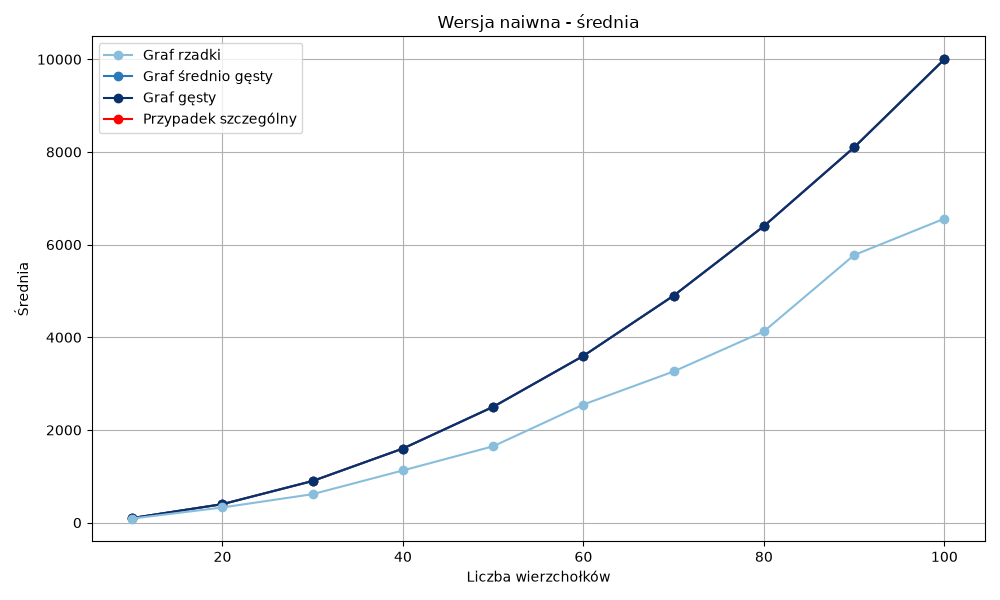
\includegraphics[width=0.9\columnwidth]{images/documentation/standard/standard_naive_mean.png}
    \caption{Średnia liczba operacji dla naiwnej wersji algorytmu Dijkstry.}
    \label{fig:standard_naive_mean}
\end{figure}

Na rys.~\ref{fig:standard_naive_mean} przedstawiono średnią liczbę operacji wykonywanych przez naiwną wersję algorytmu. Dla grafu o średniej gęstości, grafu gęstego oraz przypadku szczególnego widoczny jest ten sam wykres. Wynika to ze sposobu zliczania operacji w tej implementacji.

Podczas pojedynczej iteracji algorytmu sprawdzane jest wszystkie \(n\) wierzchołków, niezależnie od liczby krawędzi oraz ich wag. Jeżeli graf jest spójny, algorytm wykonuje \(n\) takich iteracji. Liczba zliczonych operacji jest zatem równa

\begin{equation}
C_{\mathrm{naive}} = n \cdot n = n^2.
\label{eq:naive_results_n2}
\end{equation}

Dla przykładu, dla \(n=100\) otrzymywana jest wartość

\begin{equation}
C_{\mathrm{naive}} = 100^2 = 10000,
\end{equation}

co odpowiada wartości widocznej na wykresie dla grafu średnio gęstego, gęstego oraz przypadku szczególnego.

Wyjątkiem jest graf rzadki. Jego średnia liczba operacji jest wyraźnie mniejsza od liczby operacji dla pozostałych typów grafów. Nie jest to spowodowane tym, że dla niego pojedyncza operacja wyszukiwania minimum wymagana mniejszej liczby operacji. Taki graf graf zawiera tylko

\begin{equation}
|E|=|V|
\end{equation}

krawędzi i podczas generowania nie jest wymuszane, żeby graf był spójny. Może więc powstać sytuacja, w której z wierzchołka początkowego nie da się osiągnąć wszystkich pozostałych wierzchołków.

\begin{figure}[H]
    \centering
    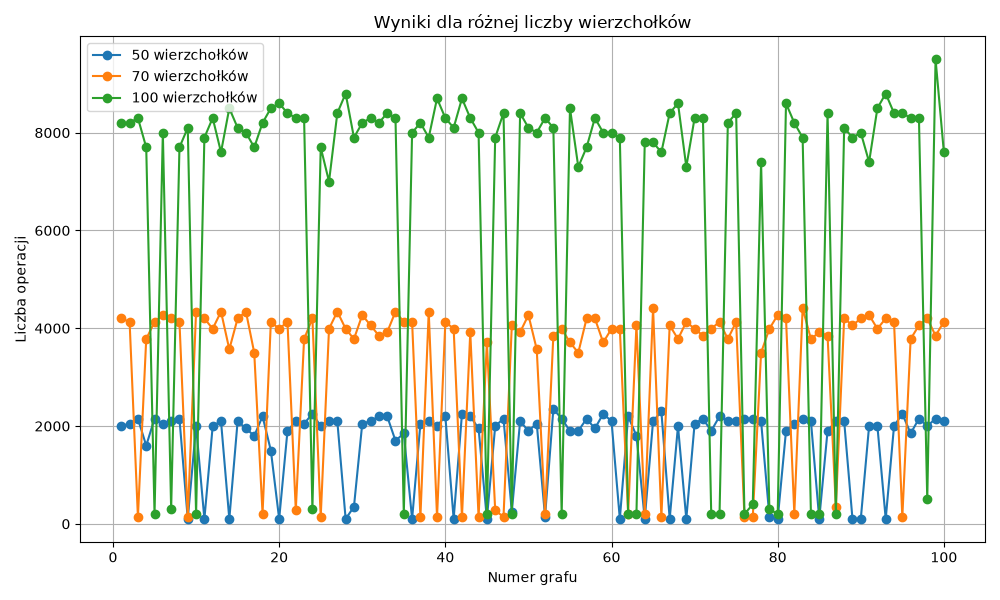
\includegraphics[width=0.95\columnwidth]{images/documentation/standard/standard_naive_verticies.png}
    \caption{Liczba operacji wersji naiwnej dla kolejnych losowo wygenerowanych grafów rzadkich.}
    \label{fig:naive_vertices_raw}
\end{figure}

Na wykresie można zauważyć wyraźny podział wyników na dwie grupy. Jednocześnie występują pojedyncze przypadki, w których liczba operacji jest bardzo mała. Takie zachowanie wynika ze struktury losowych grafów rzadkich. W wielu przypadkach wierzchołek startowy i kolejne wierzchołki są połączone z wieloma innymi. Wtedy algorytm może dotrzeć do większości wierzchołków i wykonuje dużą liczbę iteracji. Jeżeli natomiast z wierzchołka startowego lub przez jego sąsiadów nie można przejść do wielu kolejnych wierzchołków, algorytm kończy działanie znacznie wcześniej bo nie dociera do wielu wierzchołków.

Można to zauważyć na podstawie liczby operacji. Dla \(n=100\) wartości liczby operacji gdy algorytm dociera do dużej liczby wierzchołków znajdują się w okolicach \(8000\). Wynika wtedy, że stosunek liczby operacji do wierzchołków wynosi

\begin{equation}
k \approx \frac{8000}{100}=80.
\end{equation}

Oznacza to, że w tych przypadkach z wierzchołka początkowego osiągalnych jest około \(80\) spośród \(100\) wierzchołków. Analogicznie dla \(n=50\), przy wartości około \(2000\), otrzymuje się

\begin{equation}
k \approx \frac{2000}{50}=40,
\end{equation}

natomiast dla \(n=70\), przy około \(4000\) operacji,

\begin{equation}
k \approx \frac{4000}{70}\approx57.
\end{equation}

W każdym z tych przypadków osiągalnych jest około \(80\%\) wszystkich wierzchołków. Na wykresie są też przypadki, dla których koszt
jest wielokrotnie mniejszy. Odpowiadają one grafom, w których algorytm kończy działanie znacznie wcześniej.

\begin{figure}[H]
    \centering
    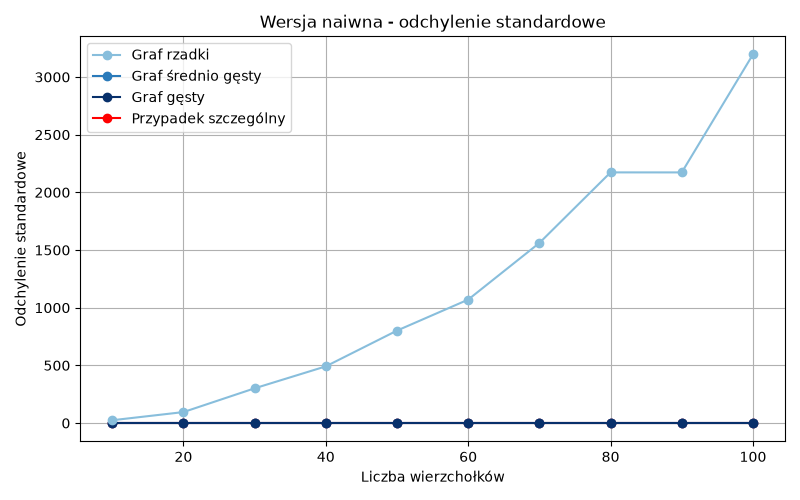
\includegraphics[width=0.9\columnwidth]{images/documentation/standard/standard_naive_std.png}
    \caption{Odchylenie standardowe liczby operacji dla naiwnej wersji algorytmu Dijkstry.}
    \label{fig:standard_naive_std}
\end{figure}

Rysunek~\ref{fig:standard_naive_std} to potwierdza. Dla grafu średnio gęstego, gęstego oraz przypadku szczególnego odchylenie standardowe wynosi zero. Każde uruchomienie dla ustalonej liczby wierzchołków wykonuje dokładnie taką samą liczbę operacji równą \(n^2\). Losowość wag i połączeń nie ma wpływu na koszt wyszukiwania w tablicy w celu znalezienia minimum.

Inaczej zachowują się grafy rzadkie. W ich przypadku widoczny jest bardzo duży wzrost odchylenia standardowego wraz ze wzrostem liczby wierzchołków. Powodem jest występowanie dwóch odległych grup wyników - tej gdzie przez algorytm jest osiągana duża liczba wierzchołków oraz drugiej gdzie algorytm kończy działanie bardzo wcześnie.

\section{Wyniki wersji z kopcem binarnym}
\label{sec:heap_results}

\begin{figure}[H]
    \centering
    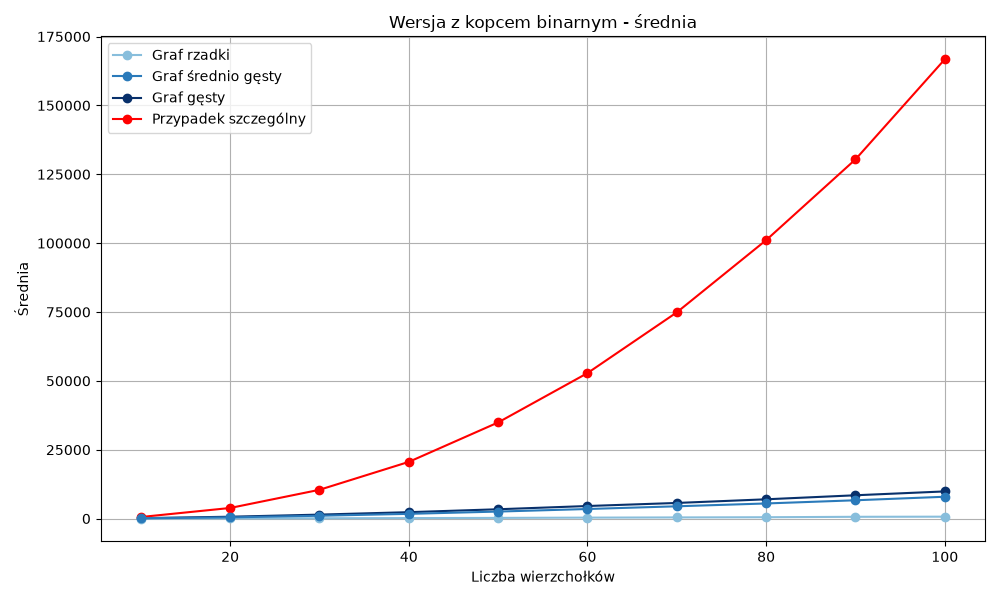
\includegraphics[width=0.9\columnwidth]{images/documentation/standard/standard_heap_mean.png}
    \caption{Średnia liczba operacji dla wersji algorytmu Dijkstry wykorzystującej kopiec binarny.}
    \label{fig:standard_heap_mean}
\end{figure}

Wyniki przedstawione na rys.~\ref{fig:standard_heap_mean} bardzo różnią się od rezultatów wersji naiwnej. Liczba operacji zależy w tym przypadku nie tylko od liczby wierzchołków, ale też od struktury grafu, wag krawędzi oraz liczby udanych relaksacji.

\subsection{Graf rzadki}

Najmniejszy średni koszt wersji z kopcem uzyskano dla grafów rzadkich, ponieważ każdy wierzchołek posiada niewielką liczbę sąsiadów. Liczba możliwości znalezienia nowej, krótszej drogi do tego samego wierzchołka jest ograniczona.

\subsection{Graf o średniej gęstości i graf gęsty}

Wraz ze wzrostem gęstości grafu zwiększa się liczba krawędzi analizowanych podczas relaksacji. Zwiększa się również liczba sytuacji, w których dla
danego wierzchołka zostaje znaleziona odległość mniejsza od wartości wyznaczonej wcześniej. Z tego powodu dla grafu średnio gęstego i gęstego liczba operacji
wykonywanych wewnątrz kopca jest znacznie większa niż w przypadku grafu rzadkiego.

\subsection{Przypadek szczególny}
\label{subsec:special_case_heap_results}

Najbardziej wyróżniającym się wynikiem jest bardzo duża liczba operacji wykonywana przez wersję z kopcem dla przypadku szczególnego. Dla \(n=100\) średnia osiąga około \(1.66\cdot10^5\) operacji, podczas gdy wersja naiwna wykonuje \(10^4\) operacji. Oznacza to ponad szesnastokrotną różnicę na korzyść wersji naiwnej.

W tym przypadku bardzo duże znaczenie ma sposób dobrania wag krawędzi. Dla przypadku szczególnego zastosowano zależność opisaną we wzorze~\eqref{eq:graph_special_case_create2}

\begin{equation}
\label{eq:graph_special_case_create2} 
w(i,j)=\begin{cases}1, & \text{gdy } j=i+1,\\[6pt]2\left(|V|-i\right), & \text{gdy } j>i+1.
\end{cases}
\end{equation}

Powoduje ona, że najkrótsza droga od wierzchołka \(0\) prowadzi kolejno przez wierzchołki

\[
0\rightarrow1\rightarrow2\rightarrow\ldots\rightarrow n-1,
\]

a odległości przyjmują wartości

\[
d(0)=0,\qquad d(1)=1,\qquad d(2)=2,\qquad \ldots,\qquad d(n-1)=n-1.
\]

Jednocześnie bezpośrednie krawędzie do dalszych wierzchołków mają duże wagi. Dzięki temu początkowo otrzymywane są duże wartości odległości, które następnie są wielokrotnie zmniejszane na etapie relaksacji.

\subsubsection{Przykład działania dla dziesięciu wierzchołków}

W celu dokładniejszego pokazania powodu dużej liczby operacji wykonywanych przez wersję wykorzystującą kopiec binarny można przeanalizować przypadek
szczególny dla \(n=10\). Przykład takiego grafu przedstawiono na rys.~\ref{fig:special_case_results_example}.

\begin{figure}[H]
    \centering
    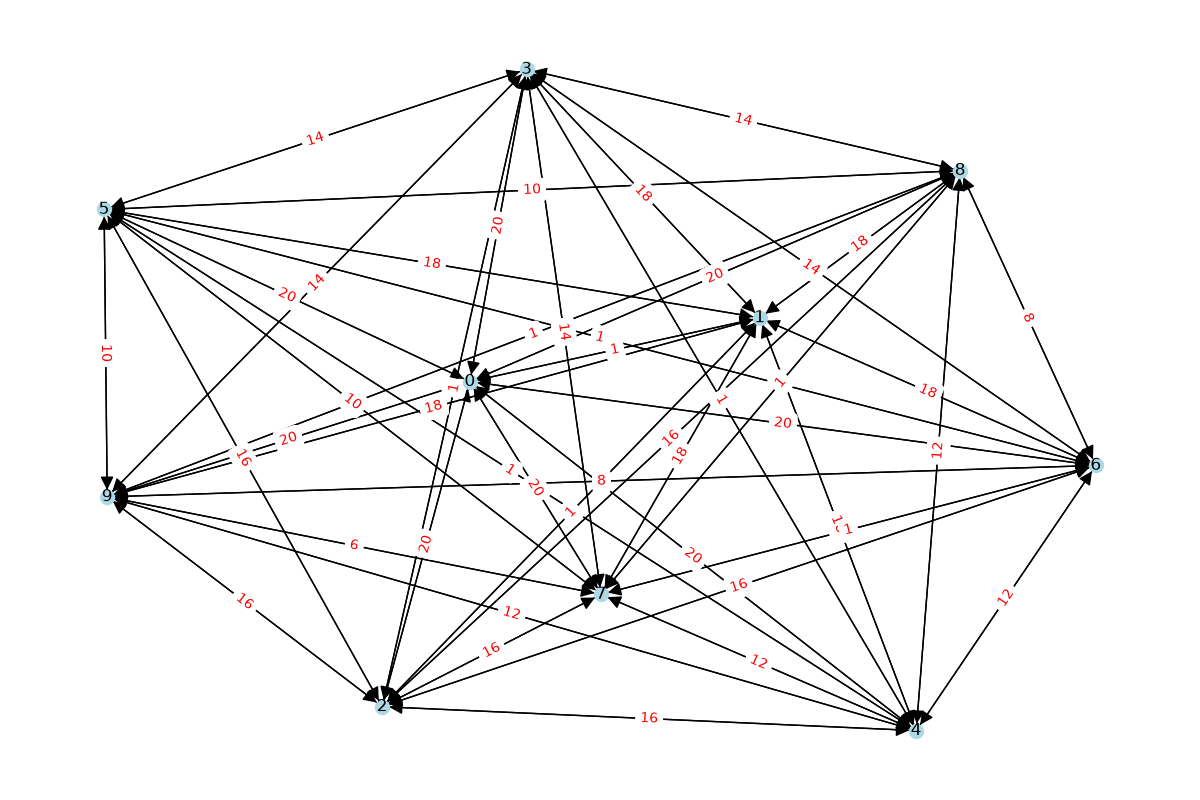
\includegraphics[width=\columnwidth]{images/documentation/graph_special_case.png}
    \caption{Przykład przypadku szczególnego dla \(10\) wierzchołków.}
    \label{fig:special_case_results_example}
\end{figure}

Wagi krawędzi w tym grafie są określone zgodnie z zależnością

\[
w(i,j)=\begin{cases}1, & \text{gdy } j=i+1,\\[4pt]2(10-i), & \text{gdy } j>i+1.
\end{cases}
\]

Oznacza to, że krawędzie łączące kolejne wierzchołki

\[
(0,1),(1,2),(2,3),\ldots,(8,9)
\]

mają wagę równą \(1\). Pozostałe krawędzie wychodzące od wierzchołka o mniejszym numerze mają odpowiednio większe wagi. Przykładowo dla
wierzchołka \(0\) wszystkie krawędzie prowadzące dalej niż do wierzchołka\(1\) mają wagę

\[
2(10-0)=20.
\]

Dla wierzchołka \(1\) odpowiednia wartość wynosi

\[
2(10-1)=18,
\]

a dla wierzchołka \(2\)

\[
2(10-2)=16,
\]

Taką zależność jest też widoczna na rys.~\ref{fig:special_case_results_example}, gdzie występują między innymi wagi \(20\), \(18\), \(16\), \(14\), \(12\), \(10\), \(8\) oraz \(6\).

Gdy algorytm rozpoczyna działanie w wierzchołku \(0\), jego początkowa odległość wynosi

\[
d(0)=0.
\]

Po przetworzeniu wierzchołka \(0\) krawędź prowadząca do wierzchołka
\(1\) ma wagę \(1\), dlatego

\[
d(1)=1.
\]

A do wszystkich pozostałych wierzchołków prowadzą krawędzie o wadze \(20\). Otrzymywane są więc odległości

\[
d(2)=d(3)=\ldots=d(9)=20.
\]

Po pierwszej relaksacji w kopcu znajdują się zatem między innymi wpisy

\[
(1,1),(20,2),(20,3),\ldots,(20,9).
\]

Najmniejszą wartość jest dla \((1,1)\), dlatego jako następny sprawdzany jest wierzchołek \(1\).

Krawędź \((1,2)\) ma wagę \(1\), zatem odległość do wierzchołka \(2\) zostaje poprawiona z \(20\) do

\[
d(2)=d(1)+1=2.
\]

Dla wszystkich dalszych wierzchołków \(j>2\) waga krawędzi wychodzącej z wierzchołka \(1\) wynosi \(18\). Nowy kandydat na odległość ma więc wartość

\[
d(1)+18=1+18=19.
\]

Otrzymuje się zatem

\[
d(3)=d(4)=\ldots=d(9)=19.
\]

Wszystkie te wartości są mniejsze od wcześniejszej wartości \(20\). Do kopca dodawane są więc nowe wpisy

\[
(2,2),(19,3),(19,4),\ldots,(19,9).
\]

W tym miejscu ujawnia się istotna cecha implementacji \textit{lazy heap}. Poprzednie elementy

\[
(20,2),(20,3),\ldots,(20,9)
\]

nie są usuwane z kopca. Pozostają w nim jako wpisy nieaktualne.

Następnie z kopca pobierany jest wierzchołek \(2\), którego poprawna odległość wynosi

\[
d(2)=2.
\]

Krawędź \((2,3)\) ma wagę \(1\), dlatego

\[
d(3)=3.
\]

Dla wierzchołków \(4,\ldots,9\) waga odpowiednich krawędzi wychodzących z wierzchołka \(2\) wynosi

\[
2(10-2)=16.
\]

Nowa odległość wynosi zatem

\[
d(2)+16=2+16=18.
\]

Wcześniej wartości te były równe \(19\), dlatego ponownie następuje udana relaksacja:

\[
d(4)=d(5)=\ldots=d(9)=18.
\]

Do kopca trafia więc kolejny zestaw elementów

\[
(3,3),(18,4),(18,5),\ldots,(18,9).
\]

Jednocześnie znajdują się w nim nadal wcześniejsze wpisy z odległościami \(19\) oraz \(20\).

Po przetworzeniu wierzchołka \(3\) sytuacja znowu się powtarza. Otrzymywana jest odległość

\[
d(4)=4,
\]

a dla wierzchołków \(5,\ldots,9\)

\[
d(j)=d(3)+2(10-3)=3+14=17.
\]

Poprzednia wartość wynosiła \(18\), dlatego wszystkie te odległości ponownie zostają poprawione.

Pierwsze etapy działania algorytmu można więc przedstawić w ten sposób:

\begin{center}
\begin{tabularx}{\textwidth}{
    >{\hsize=.7\hsize\centering\arraybackslash}X |
    >{\hsize=1.15\hsize\centering\arraybackslash}X |
    >{\hsize=1.15\hsize\centering\arraybackslash}X
}
\textbf{przetworzony wierzchołek} &
\textbf{odległość do następnego wierzchołka} &
\textbf{odległość do dalszych wierzchołków} \\ \hline
0 & \(d(1)=1\) & 20 \\
1 & \(d(2)=2\) & 19 \\
2 & \(d(3)=3\) & 18 \\
3 & \(d(4)=4\) & 17 \\
4 & \(d(5)=5\) & 16 \\
5 & \(d(6)=6\) & 15 \\
6 & \(d(7)=7\) & 14 \\
7 & \(d(8)=8\) & 13 \\
8 & \(d(9)=9\) & 12 \\
\end{tabularx}
\end{center}
Widoczny jest więc mechanizm działania algorytmu na przygotowanym grafie. Przetworzenie kolejnego wierzchołka powoduje poprawienie odległości do prawie wszystkich wierzchołków znajdujących się dalej w kolejności. Wartość kandydata zmniejsza się przy tym o \(1\) w stosunku do wartości uzyskanej w poprzedniej iteracji.

Dla przykładu odległość do wierzchołka \(9\) jest aktualizowana wielokrotnie:

\[
20 \rightarrow 19 \rightarrow 18 \rightarrow 17 \rightarrow 16 \rightarrow 15 \rightarrow 14\rightarrow 13 \rightarrow 9.
\]

To samo jest dla pozostałych dalszych wierzchołków. Dlatego ten sam wierzchołek posiada w kopcu wiele wpisów odpowiadających kolejnym, coraz mniejszym odległościom.

Przykładowo dla wierzchołka \(9\) w trakcie działania algorytmu mogą pojawić się wpisy

\[
(20,9),\;(19,9),\;(18,9),\;(17,9),\;(16,9),\;(15,9),\;(14,9),\;(13,9),\;(9,9).
\]

Tylko ostatni z nich odpowiada ostatecznej najkrótszej odległości. Pozostałe elementy stają się wpisami nieaktualnymi, jednak nadal znajdują się w kopcu. Dlatego pobieranie nowych elementów z kopca staje się coraz bardziej kosztowne. Powoduje ono wiele operacji przesuwania elementów w celu przywrócenia własności kopca.

\subsection{Odchylenie standardowe wersji z kopcem}

\begin{figure}[H]
    \centering
    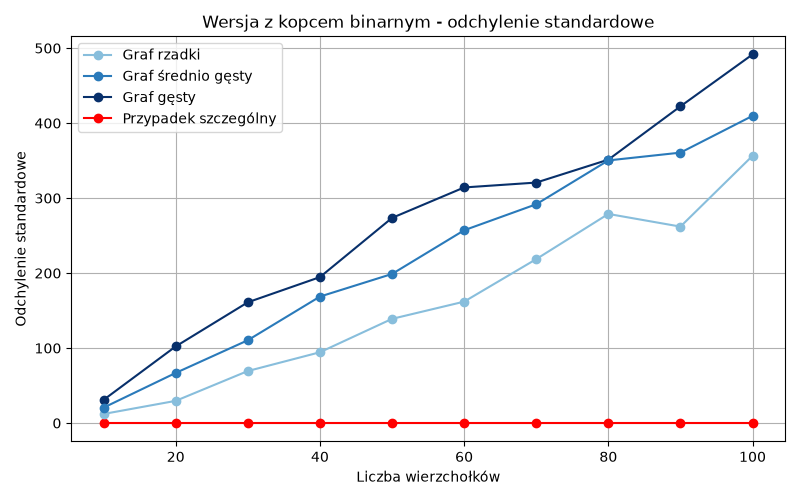
\includegraphics[width=0.9\columnwidth]{images/documentation/standard/standard_heap_std.png}
    \caption{Odchylenie standardowe liczby operacji dla wersji wykorzystującej kopiec binarny.}
    \label{fig:standard_heap_std}
\end{figure}

Na rys.~\ref{fig:standard_heap_std} widoczny jest wzrost odchylenia standardowego dla trzech losowo generowanych typów grafów. Jest to konsekwencją losowego doboru krawędzi, jak i ich wag.

W przypadku grafu średnio gęstego i gęstego różne wagi prowadzą do różnej liczby udanych relaksacji. Jeżeli pierwsza znaleziona droga do wierzchołka jest już stosunkowo krótka, liczba kolejnych aktualizacji wag będzie niewielka. Jeżeli natomiast początkowo znaleziona zostanie droga o dużym koszcie, może być ona poprawiana wielokrotnie. Każda poprawa powoduje wstawienie nowego elementu do kopca i zwiększa całkowitą liczbę operacji. Dla grafu rzadkiego dodatkowym czynnikiem jest fakt że wygenerowany graf rzadki nie zawsze jest spójny. 

\begin{figure}[H]
    \centering
    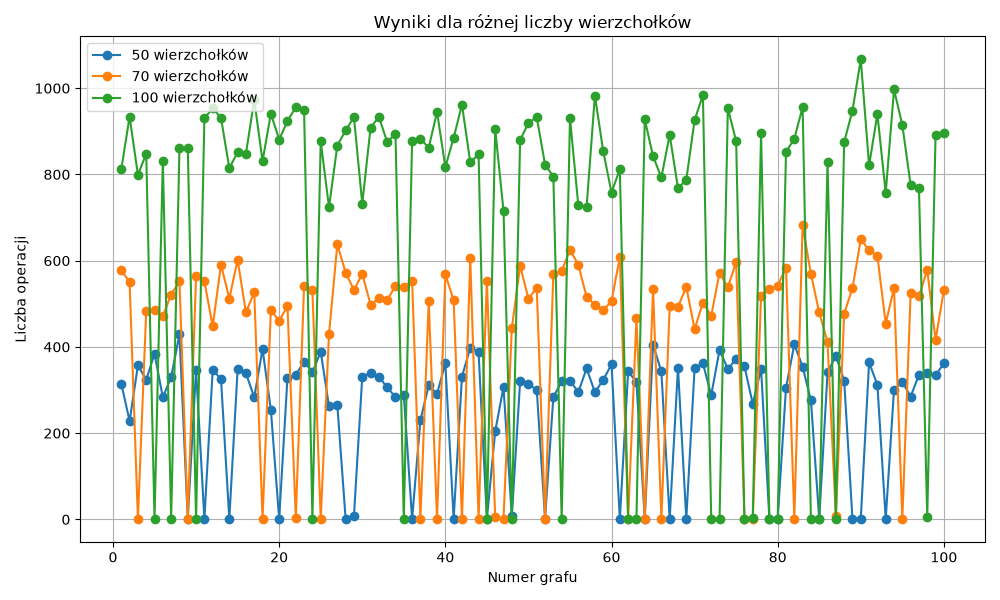
\includegraphics[width=0.95\columnwidth]{images/documentation/standard/standard_heap_verticies.png}
    \caption{Liczba operacji wersji z kopcem binarnym dla kolejnych losowo wygenerowanych grafów rzadkich.}
    \label{fig:heap_vertices_raw}
\end{figure}

Jak pokazano na rys.~\ref{fig:heap_vertices_raw}, podobnie jak w przypadku wersji naiwnej, wyniki tworzą dwie wyraźne grupy. Dla \(100\) wierzchołków duża część wyników znajduje się w przedziale około \(800\)--\(950\) operacji, a część przyjmuje wartości bliskie zeru lub znacznie mniejsze od głównej grupy. Dla \(70\) wierzchołków dominują wartości około \(500\)--\(600\), a dla \(50\) wierzchołków około \(300\)--\(350\).

W przypadku szczególnym odchylenie standardowe wynosi dokładnie zero bo nie występuje tam losowanie struktury ani wag grafu. Dla ustalonego \(n\) każdy wygenerowany przypadek ma dokładnie ten sam układ krawędzi i wag, a algorytmu wykonuje tę samą liczbę operacji. 

\section{Bezpośrednie porównanie średnich wartości}

\begin{figure}[H]
    \centering
    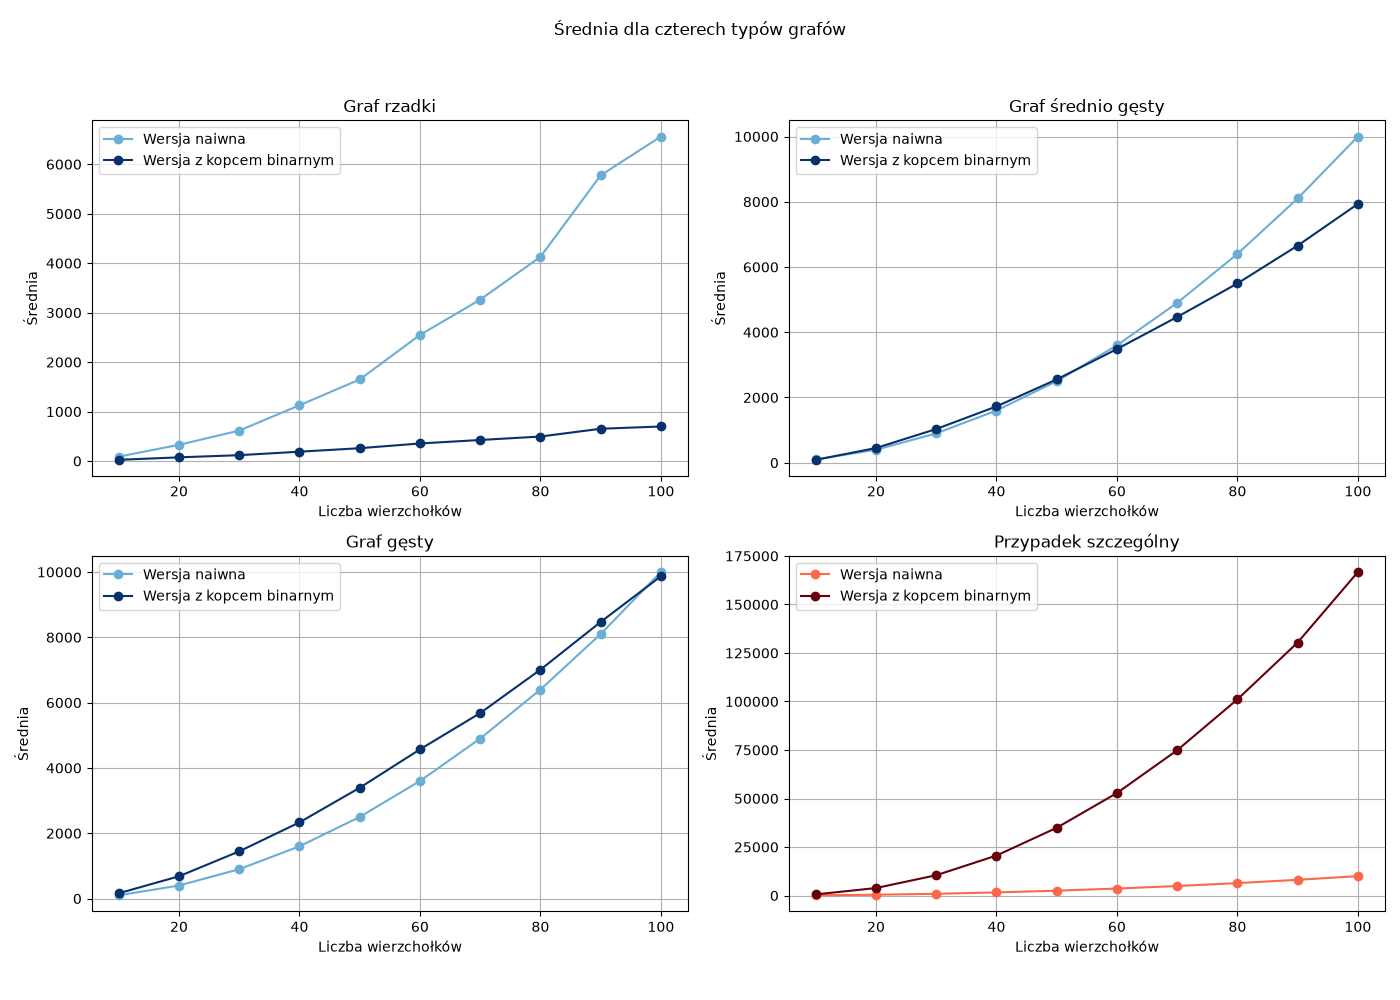
\includegraphics[width=\columnwidth]{images/documentation/standard/standard_naive_vs_std_mean_graph_types.png}
    \caption{Porównanie średniej liczby operacji wersji naiwnej i wersji z kopcem dla poszczególnych typów grafów.}
    \label{fig:standard_mean_graph_types}
\end{figure}

Rysunek~\ref{fig:standard_mean_graph_types} pozwala bezpośrednio porównać obie implementacje dla każdego rodzaju grafu.

Dla grafu rzadkiego zastosowanie kopca przynosi największą korzyść. Niewielka liczba krawędzi ogranicza liczbę relaksacji, czyli też liczbę nowych wpisów umieszczanych w kopcu. Na tym samym grafie wersja naiwna przy każdej iteracji nadal przegląda całą tablicę wierzchołków. W przypadku grafu o średniej gęstości przewaga kopca jest mniejsza jednak powiększa się ona wraz ze wzrostem liczby krawędzi. Natomiast dla grafu gęstego wartości obu wariantów stają się do siebie zbliżone a dla 100 wierzchołków wersja naiwna zaczyna być lepsza od kopcowej. Wynika to z coraz większej liczby relaksacji przy zwiększającej się liczbie wierzchołków. Zupełnie inne wyniki widoczne są dla przypadku szczególnego. Wersja naiwna pozostaje na poziomie \(n^2\), a koszt wersji z kopcem bardzo szybko rośnie. Dla \(n=100\) wartości wynoszą odpowiednio około

\[
10000
\]

oraz

\[
166000.
\]

Stosunek tych wartości wynosi w przybliżeniu

\begin{equation}
\frac{166000}{10000}\approx16.6.
\end{equation}

Oznacza to, że w algorytm wykorzystujący kopiec wykonuje w tym przypadku około \(16.6\) razy więcej operacji niż w wersji naiwnej.

\begin{figure}[H]
    \centering
    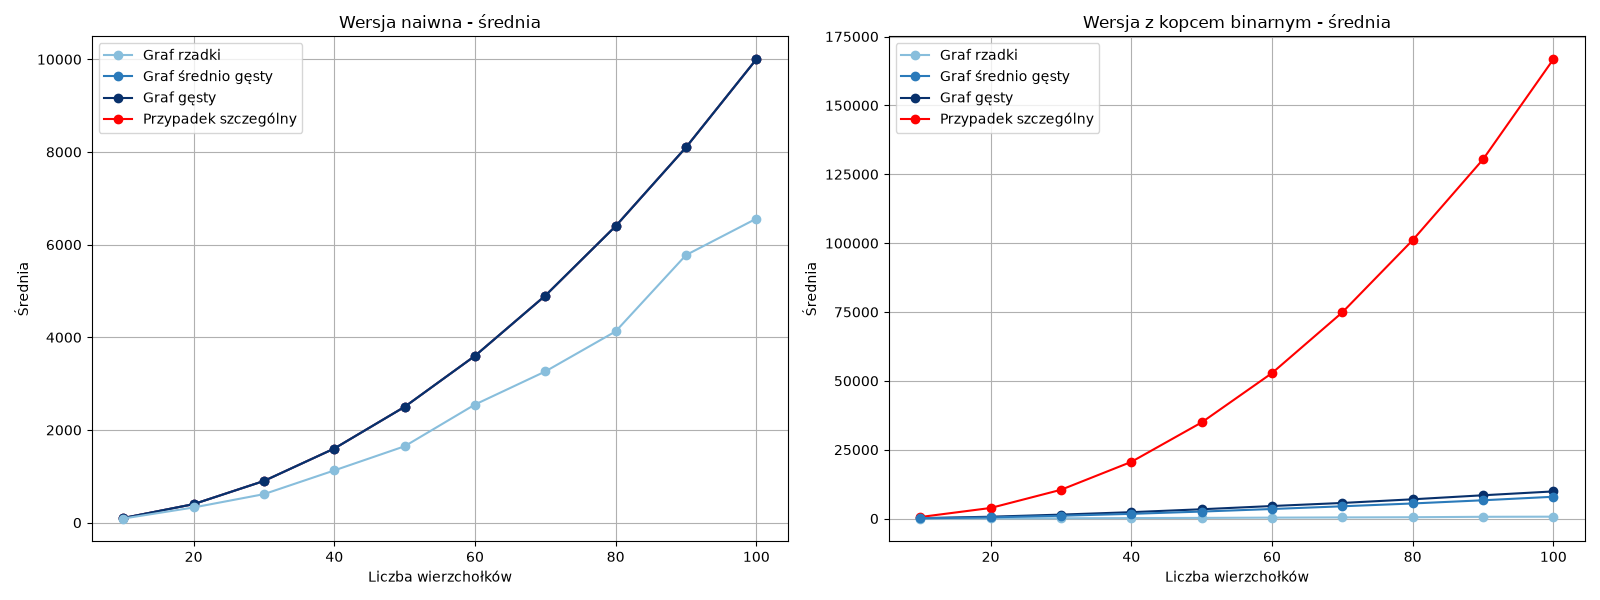
\includegraphics[width=\columnwidth]{images/documentation/standard/standard_naive_vs_std_mean.png}
    \caption{Porównanie średniej liczby operacji dla wszystkich typów grafów i obu implementacji.}
    \label{fig:standard_mean_comparison}
\end{figure}

Na rys.~\ref{fig:standard_mean_comparison} jeszcze lepiej jest widoczna różnica pomiędzy przypadkiem szczególnym a pozostałymi grafami. 

\section{Porównanie odchylenia standardowego}

\begin{figure}[H]
    \centering
    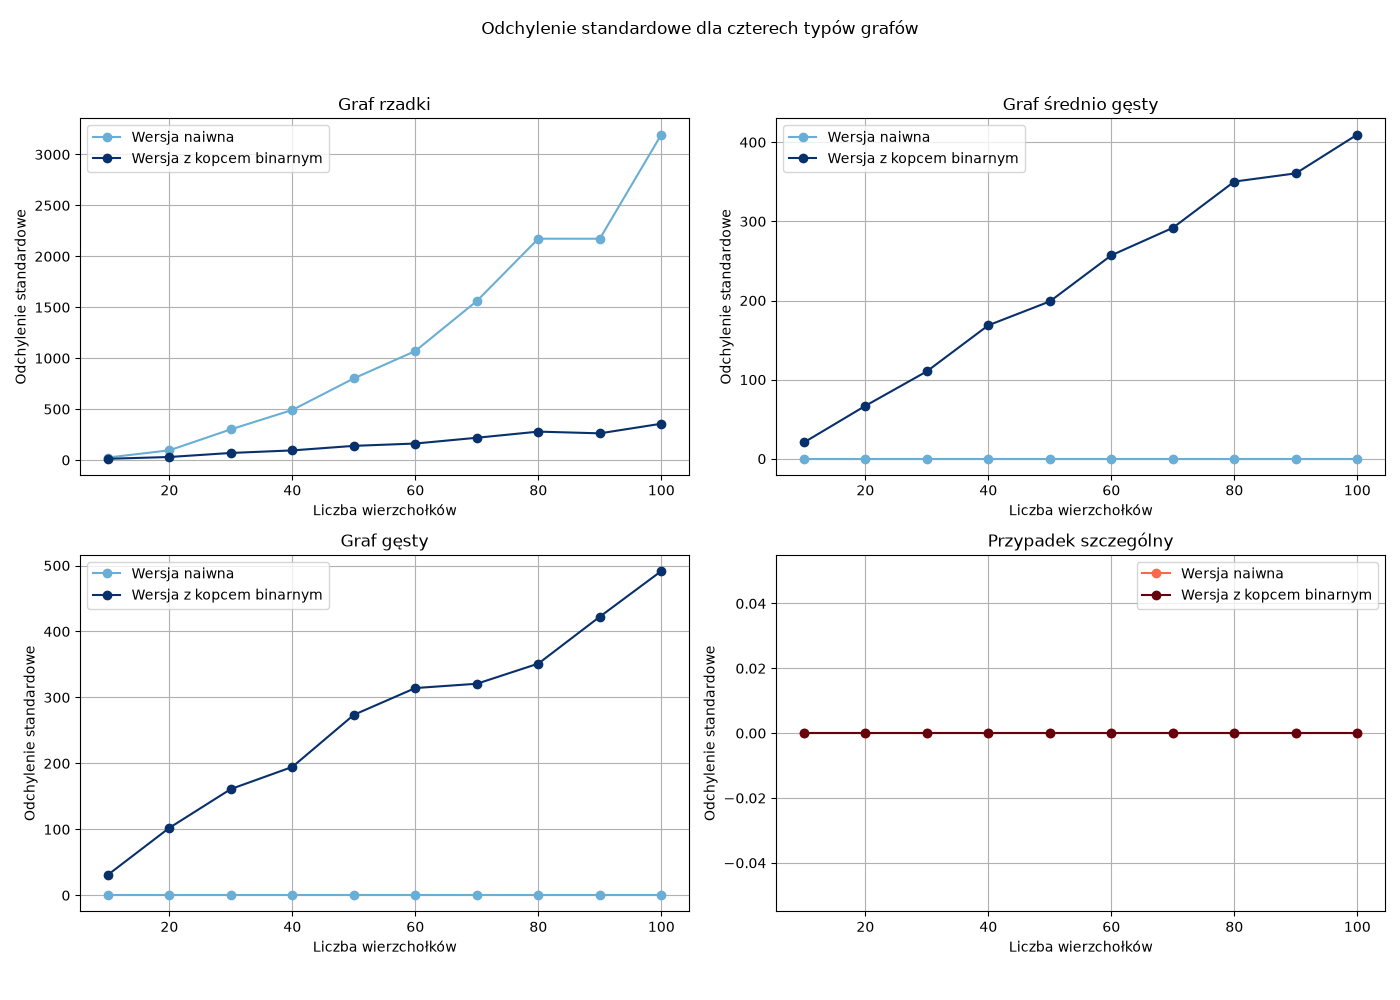
\includegraphics[width=\columnwidth]{images/documentation/standard/standard_naive_vs_std_std_graph_types.png}
    \caption{Porównanie odchylenia standardowego obu implementacji dla poszczególnych typów grafów.}
    \label{fig:standard_std_graph_types}
\end{figure}

\begin{figure}[H]
    \centering
    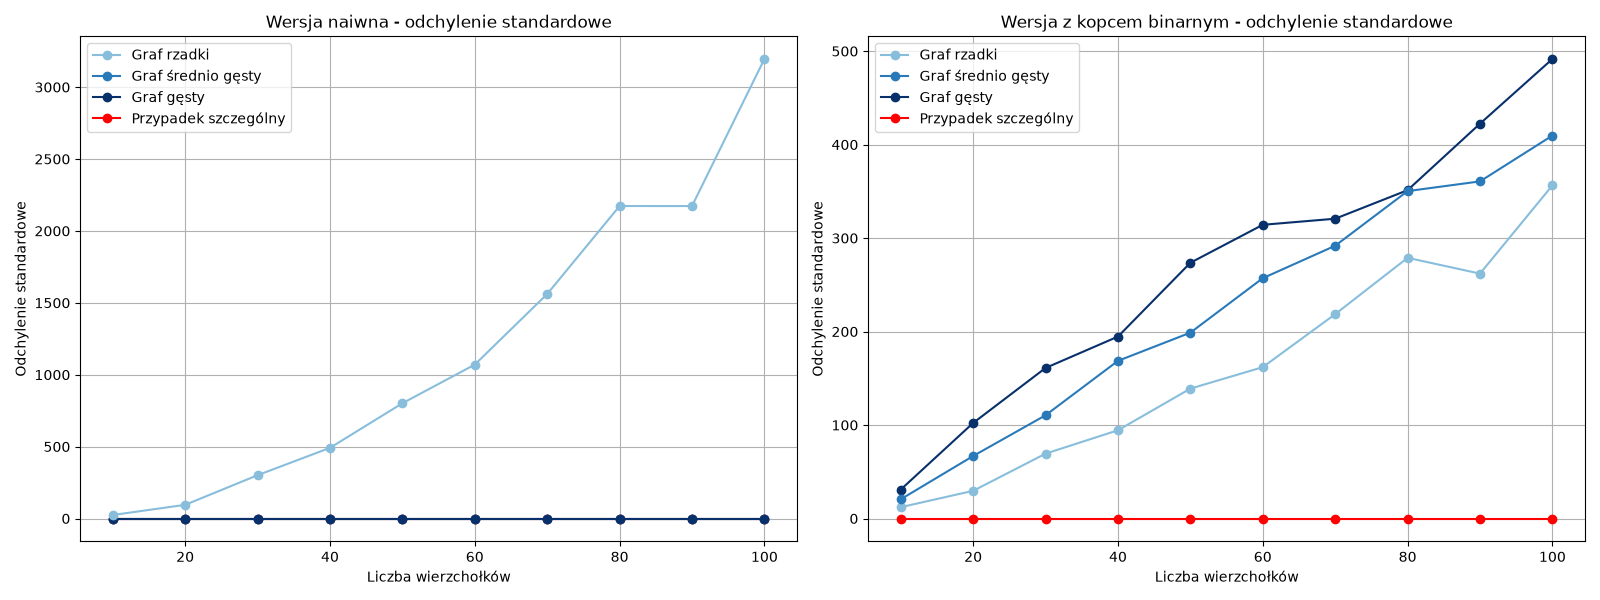
\includegraphics[width=\columnwidth]{images/documentation/standard/standard_naive_vs_std_std.png}
    \caption{Porównanie odchylenia standardowego dla wszystkich typów grafów.}
    \label{fig:standard_std_comparison}
\end{figure}

Rysunki~\ref{fig:standard_std_graph_types}
i~\ref{fig:standard_std_comparison} bardzo dobrze pokazują różnicę pomiędzy stabilnością obu metod zliczania.

W wersji naiwnej dla grafów spójnych liczba operacji zależy wyłącznie od liczby wierzchołków. Dla grafu średnio gęstego, gęstego i przypadku szczególnego odchylenie standardowe wynosi zero. Jedynie dla grafu rzadkiego odchylenie standardowe jest bardzo duże. Na podstawie rys.~\ref{fig:naive_vertices_raw} można stwierdzić, że jest on spowodowany różnicami pomiędzy losowymi grafami. Czasami algorytm kończy działanie bardzo wcześnie bo nie może dotrzeć do wielu wierzchołków.

W wersji z kopcem wyniki zależą znacznie bardziej od konkretnego układu wag i liczby udanych relaksacji. Nawet dla grafów o tej samej liczbie wierzchołków i krawędzi różna kolejność poprawiania odległości może spowodować inną liczbę operacji wstawiania i pobierania wierzchołków z kopca. W przypadku grafu rzadkiego dodatkowo występuje ten sam efekt związany z brakiem spójności grafów co w wersji naiwnej. Powoduje to występowanie zarówno bardzo niskich i wysokich wyników, co jest widoczne na rys.~\ref{fig:heap_vertices_raw}.

Natomiast dla przypadku szczególnego zarówno w wersji z kopcem jak i naiwnej odchylenie standardowe jest równe zeru. Jest to spowodowane specyficzną konstrukcją grafu która wymuszając maksymalną liczbę relaksacji poprzez odpowiedni dobór wag sprawia że algorytm działa zawsze w ten sam powtarzalny sposób.
